\documentclass{article}

\usepackage{fancyhdr}
\usepackage{extramarks}
\usepackage{amsmath}
\usepackage{amsthm}
\usepackage{amsfonts}
\usepackage{tikz}
\usepackage[plain]{algorithm}
\usepackage{algpseudocode}
\usepackage{listings}
\usepackage{minted}
\usepackage[utf8]{inputenc}
\usepackage[english]{babel}
\usetikzlibrary{automata,positioning}
\usepackage{graphicx}
\usepackage{amsmath}
\usepackage{tikz}
\usetikzlibrary{positioning}
%
% Basic Document Settings
%


\topmargin=-0.45in
\evensidemargin=0in
\oddsidemargin=0in
\textwidth=6.5in
\textheight=9.0in
\headsep=0.25in

\linespread{1.1}

\pagestyle{fancy}
\lhead{\hmwkClass\ (\hmwkClassInstructor): \hmwkTitle}
\chead{\hspace{4.8in}\hmwkAuthorName}
\rhead{\firstxmark}
\lfoot{\lastxmark}
\cfoot{\thepage}

\renewcommand\headrulewidth{0.4pt}
\renewcommand\footrulewidth{0.4pt}

\setlength\parindent{0pt}

%
% Create Problem Sections
%

\newcommand{\enterProblemHeader}[1]{
    \nobreak\extramarks{}{Problem \arabic{#1} continued on next page\ldots}\nobreak{}
    \nobreak\extramarks{Problem \arabic{#1} (continued)}{Problem \arabic{#1} continued on next page\ldots}\nobreak{}
}

\newcommand{\exitProblemHeader}[1]{
    \nobreak\extramarks{Problem \arabic{#1} (continued)}{Problem \arabic{#1} continued on next page\ldots}\nobreak{}
    \stepcounter{#1}
    \nobreak\extramarks{Problem \arabic{#1}}{}\nobreak{}
}

\setcounter{secnumdepth}{0}
\newcounter{partCounter}


%
% Homework Problem Environment
%
% This environment takes an optional argument. When given, it will adjust the
% problem counter. This is useful for when the problems given for your
% assignment aren't sequential. See the last 3 problems of this template for an
% example.
%


%
% Homework Details
%   - Title
%   - Due date
%   - Class
%   - Section/Time
%   - Instructor
%   - Author
%

\newcommand{\hmwkTitle}{Homework 4}
\newcommand{\hmwkDueDate}{Tuesday, March 22, 2016}
\newcommand{\hmwkClass}{DS-GA 1003}
\newcommand{\hmwkClassInstructor}{Professor David Ronsenberg}
\newcommand{\hmwkAuthorName}{Yuhao Zhao}
\newcommand{\hmwknetid}{Yz3085}
\newcommand{\hmwksubtitle}{Kernels, Duals, and Trees}
\newcommand{\gihub}{See complete code at: \textit{git@github.com:cryanzpj/1003.git}}
%
% Title Page
%

\title{
    \vspace{2in}
    \textmd{\textbf{\hmwkClass:\ \hmwkTitle \\ \hmwksubtitle }}\\
    \vspace{1in}
    \normalsize\vspace{0.1in}\small{Due\ on\ \hmwkDueDate}\\
    \vspace{0.1in}\large{\textit{\hmwkClassInstructor}}\\
    \vspace{3in}
    \author{\textbf{\hmwkAuthorName} \\ \textbf{\hmwknetid }\\ }
    \vspace{0.2in}
    \gihub
}



\date{}

\renewcommand{\part}[1]{\textbf{\large Part \Alph{partCounter}}\stepcounter{partCounter}\\}

%
% Various Helper Commands
%

% Useful for algorithms
\newcommand{\alg}[1]{\textsc{\bfseries \footnotesize #1}}

% For derivatives
\newcommand{\deriv}[1]{\frac{\mathrm{d}}{\mathrm{d}x} (#1)}

% For partial derivatives
\newcommand{\pderiv}[2]{\frac{\partial}{\partial #1} (#2)}

% Integral dx
\newcommand{\dx}{\mathrm{d}x}

% Alias for the Solution section header
\newcommand{\solution}{\textbf{\large Solution}}

% Probability commands: Expectation, Variance, Covariance, Bias
\newcommand{\E}{\mathrm{E}}
\newcommand{\Var}{\mathrm{Var}}
\newcommand{\Cov}{\mathrm{Cov}}
\newcommand{\Bias}{\mathrm{Bias}}





\newenvironment{problem}[2][$\bullet$]{\begin{trivlist}\large
		\item[\hskip \labelsep {\bfseries #1}\hskip \labelsep {\bfseries #2.}]}  {\end{trivlist}}

\newenvironment{sub}[2][$-$]{\begin{trivlist}
		\item[\hskip \labelsep {\bfseries #1}\hskip \labelsep {\bfseries #2.}]}  {\end{trivlist}}
\newenvironment{lemma}[2][Lemma]{\begin{trivlist}
		\item[\hskip \labelsep {\bfseries #1}\hskip \labelsep {\bfseries #2.}]}{\end{trivlist}}
\newenvironment{exercise}[2][Exercise]{\begin{trivlist}
		\item[\hskip \labelsep {\bfseries #1}\hskip \labelsep {\bfseries #2.}]}{\end{trivlist}}

\newenvironment{question}[2][Question]{\begin{trivlist}
		\item[\hskip \labelsep {\bfseries #1}\hskip \labelsep {\bfseries #2.}]}{\end{trivlist}}
\newenvironment{corollary}[2][Corollary]{\begin{trivlist}
		\item[\hskip \labelsep {\bfseries #1}\hskip \labelsep {\bfseries #2.}]}{\end{trivlist}}

\begin{document}

\maketitle

\pagebreak

\section{2 Positive Semidefinite Matrices}

\begin{sub}{2.1}
\end{sub}
Let $A = \frac{1}{\sqrt{2}} \begin{bmatrix} 1 & 1\\ -1&1 \end{bmatrix} ,
 A^TA = \frac{1}{2} \begin{bmatrix} 1 & 1\\ -1&1 \end{bmatrix} \begin{bmatrix} 1 & -1\\ 1& 1 \end{bmatrix}  = \begin{bmatrix} 1 & 0\\ 0&1 \end{bmatrix}  $ and A is not symmetric.\\
 
 \begin{sub}{2.2}
 \end{sub}
 Since M is psd, we assume M is real and symmetric, thus by Spectral Theorem, we have $$M = Q\Sigma Q^T$$ where Q is an orthogonal matrix ($Q^T = Q^{-1}$), $\Sigma$ is diagonal. 
 $$\Sigma  = Q^{-1} M(Q^{T})^{-1} = Q^TMQ = 
 \begin{pmatrix}q_{1}^{T}Mq_{1} & q_{1}^{T}Mq_{2} & \cdots & q_{1}^{T}Mq_{n}\\
 q_{2}^{T}Mq_{1} & q_{2}^{T}Mq_{2} & \cdots & q_{2}^{T}Mq_{n}\\
 \vdots & \vdots & \cdots & \vdots\\
 q_{d}^{T}Mq_{1} & q_{d}^{T}Mq_{2} & \cdots & q_{d}^{T}Mq_{n}
 \end{pmatrix}.
 $$
 Since M is psd, $q_i^TMq_i \geq 0$, the diagonals of $\Sigma$ are eigenvalues of M and are non-negative. 
 
 \begin{sub}{2.3}
 \end{sub}
 i). If we have  M = $BB^T$ for some B, for $\forall  v \in \Re^n$
 $$v^TMv = v^TBB^Tv = (B^Tv)^T(B^Tv) = ||B^Tv|| \geq 0$$ Therefore, M is psd\\
 ii). If we know M is psd, by spectral theorem
 $$M =  Q\Sigma Q^T = Q\Sigma^{\frac{1}{2}} \Sigma^{\frac{1}{2}} Q^T = Q\Sigma^{\frac{1}{2}}(Q\Sigma^{\frac{1}{2}})^{T} = BB^T$$
 where $B =Q\Sigma^{\frac{1}{2}}\\ \Sigma^{\frac{1}{2}}$ is a diagonal matrix whose diagonal equals the sqrt root of $diag(\Sigma)$\\
 
 This proves a symmetric matrix M can be expressed as $M = BB^T$ iff M is psd
 
 \section{3 Positive Definite Matrices}
 
 \begin{sub}{3.1}
 \end{sub}
 M is pd, by Spectral Theorem, $$M = Q\Sigma Q^T$$
 $$\Sigma  = Q^{-1} M(Q^{T})^{-1} = Q^TMQ = 
 \begin{pmatrix}q_{1}^{T}Mq_{1} & q_{1}^{T}Mq_{2} & \cdots & q_{1}^{T}Mq_{n}\\
 q_{2}^{T}Mq_{1} & q_{2}^{T}Mq_{2} & \cdots & q_{2}^{T}Mq_{n}\\
 \vdots & \vdots & \cdots & \vdots\\
 q_{d}^{T}Mq_{1} & q_{d}^{T}Mq_{2} & \cdots & q_{d}^{T}Mq_{n}
 \end{pmatrix}.
 $$ Since M is pd, $q_i^TMq_i > 0$, the diagonals of $\Sigma$ are eigenvalues of M and are positive . 

\pagebreak

\begin{sub}{3.2}
\end{sub}
since M is positive definite, $M = Q\Sigma Q^T$
$$Q\Sigma Q^{T} M = Q\Sigma^{-1} Q^T Q\Sigma Q^T$$
Q is an orthogonal matrix, $Q^TQ = I$ 
$$ RHS = Q\Sigma^{-1} \Sigma  Q^T = QQ^T = I $$
Therefore, $Q\Sigma Q^{T}$ is the inverse of M

\begin{sub}{3.3}
\end{sub}

M is psd and symmetric, for $\forall  v \in \Re^n ,v \neq \vec{0}, \text{and } \lambda >0$
$$v^T(M+\lambda I ) v = v^TMv + \lambda v^Tv > 0$$
since $v^TMv \geq 0, \lambda v^Tv > 0$. Therefore, $v^T(M+\lambda I ) v$ is positive definite. \\
To show, $M+\lambda I  $ is symmetric, we know that $\forall i \neq j, (M+\lambda I )_{i,j} = M_{i,j} = M_{j,i} = (M+\lambda I )_{j,i}$. Thus $M+\lambda I  $  is also symmetric. \\

let $v_1,...,v_n, \lambda_1, ..., \lambda_n$ be the n eigenvalues and  eigenvectors of M 
$$ (M+\lambda I ) v_i = Mv_i + \lambda v_i = \lambda_i v_i + \lambda v_i  = (\lambda_i + \lambda) v_i$$
Therefore, $v_i$ is also a eigenvector of $M+\lambda I$ with corresponding eigenvalue equals to $(\lambda_i + \lambda)$.\\
$M+\lambda I  = Q\Sigma Q^T, Q = \{v_1,...,v_n\}, \Sigma_{i,i} = \lambda_i + \lambda$, Then we have 
$$(M+\lambda I )^{-1} = (Q^T)^{-1} \Sigma^{-1} Q^{-1} = Q \Sigma^{-1} Q^T = \sum_{i=1}^{n} \frac{1}{\lambda_i+\lambda} v_iv_i^T$$

\begin{sub}{3.4}
\end{sub}

M is symmetric psd and N is symmetric pd, $\forall  v \in \Re^n ,v \neq \vec{0}$
$$v^T(M+N)v = v^TMv + v^TNv$$
we know $v^TMv \geq 0, v^TNv > 0 $
$$v^T(M+N)v > 0 $$
This shows $M+N$ is positive definite. \\
To show $M+N$ is symmetric, $\forall i \neq j, (M+N)_{i,j} = M_{i,j} + N_{i,j} = M_{j,i} + N_{j,i} = (M+N)_{j,i}$ , Thus $M+N$ is also symmetric. 
From 3.2 we know that positive definite matrix has inverse. Therefore, M+N is invertible. 

\section{4 Kernel Matrices}
$$K = XX^T = \begin{pmatrix}
x_1^Tx_1 & \cdots & x_1^Tx_m\\
\vdots&\vdots &\vdots\\
x_m^Tx_1 & \cdots &x_m^Tx_m
\end{pmatrix}$$
$d(x_i,x_j) = ||x_i - x_j|| = \sqrt{(x_i - x_j)\cdot (x_i - x_j)} = \sqrt{x_i\cdot x_i + x_j \cdot x_j -2 x_i \cdot x_j} = \sqrt{K_{i,i} + K_{j,j} - 2 K_{i,j}}$\\
Therefore , knowing K is equivalent to knowing the set of pairwise distance of vectors in S.

\pagebreak 

\section{5 Kernel Ridge Regression}
\begin{sub}{5.1}
\end{sub}
Since 
\begin{align}
J(w)  &= ||Xw - y|| + \lambda ||w^2||\\
\frac{\partial J}{\partial w} &= 2X^T(Xw - y) + 2\lambda wI = 0
\end{align}

we have \begin{align}
X^TXw - X^Ty + \lambda wI & = (X^TX+\lambda I)w - X^Ty= 0\\
w^* &= (X^TX+\lambda I)^{-1} X^Ty
\end{align}
$XX^T$ is positive semidefinite and $\lambda >0$, by 3.3, $XX^T + \lambda I$ is positive definite, thus invertible. 

\begin{sub}{5.2}
\end{sub}

Since $X^TXw + \lambda I w = X^Ty, w = \frac{1}{\lambda}(X^Ty - X^TXw) =  X^T\frac{1}{\lambda}(y - Xw)$\\
Thus $w = X^T\alpha$, where $\alpha =\frac{1}{\lambda}(y - Xw) $

\begin{sub}{5.3}
\end{sub}
Since $w = X^T\alpha = \sum_{1}^{n} \alpha_i x_i$, w is a linear combination of data vectors 

\begin{sub}{5.4}
\end{sub}
since $w = X^T\alpha$ and $X^TXw + \lambda I w = X^Ty$
\begin{align}
X^TXX^T\alpha + \lambda I X^T\alpha &= X^Ty\\
X^T(XX^T+\lambda I)\alpha &= X^Ty\end{align}
Therefore $\alpha = (XX^T+\lambda I)^{-1}y$

\begin{sub}{5.5}
\end{sub}
Since $w = X^T\alpha = X^T(XX^T+\lambda I)^{-1}y, XX^T = K$
\begin{align} Xw &= XX^T(XX^T+\lambda I)^{-1}y \\ &= K(K+\lambda I )^{-1} y 
\end{align}

\begin{sub}{5.6}
\end{sub}

For a new point $\tilde{x}$

\begin{align}
\tilde{x}^T w^* &= \tilde{x}^TX^T(K+\lambda I)^{-1}y\\
&= \begin{pmatrix}
\tilde{x}^Tx_1 & \tilde{x}^Tx_2 & \cdots & \tilde{x}^Tx_n
\end{pmatrix}(K+\lambda I)^{-1}y\\
&= k_{\tilde{x}}^T(K+\lambda I)^{-1}y\
\end{align}


\pagebreak

\section{6 Decision Trees}

\begin{problem}{6.1 Building Trees by Hand}
\end{problem}
\begin{sub}{6.1.1}
\end{sub}
a) Split on size: 

i) Size $\leq 1$, 
$p_1 = \frac{2}{3} ,N_1 = 3,Q_1 = \frac{4}{9},  p_2 = \frac{3}{8},N_2 = 8, Q_2= \frac{30}{64}, N_1Q_1 + N_2Q_2 = \frac{61}{12} \approx 5.08$\\
ii) Size $\leq 2$,
$p_1 = \frac{2}{5} ,N_1 = 5,Q_1 = \frac{12}{25},  p_2 = \frac{3}{6},N_2 = 6, Q_2= \frac{18}{36}, N_1Q_1 + N_2Q_2  \approx 5.4$\\
iii) Size $\leq 3$,
$p_1 = \frac{2}{6} ,N_1 = 6,Q_1 = \frac{16}{36},  p_2 = \frac{3}{5},N_2 = 5, Q_2= \frac{12}{25}, N_1Q_1 + N_2Q_2  \approx 5.06$\\
iv) Size $\leq 4$,
$p_1 = \frac{4}{9} ,N_1 = 9,Q_1 = \frac{40}{81},  p_2 = \frac{1}{2},N_2 = 2, Q_2= \frac{1}{2}, N_1Q_1 + N_2Q_2  \approx 5.4$\\

b) split on spots:

v)  spots = N,
$p_1 = 0 ,N_1 = 4,Q_1 = 0,  p_2 = \frac{5}{7},N_2 = 7, Q_2= \frac{20}{49}, N_1Q_1 + N_2Q_2  \approx 2.85$\\

c) split on color:

vi) color = white,
$p_1 = \frac{2}{5} ,N_1 = 5,Q_1 = \frac{12}{25},  p_2 = \frac{3}{6},N_2 = 6, Q_2= \frac{18}{36}, N_1Q_1 + N_2Q_2  \approx 5.4$ \\
The minimal weighted impurity measure is obtained by splitting on the spots.  \\


\begin{center}
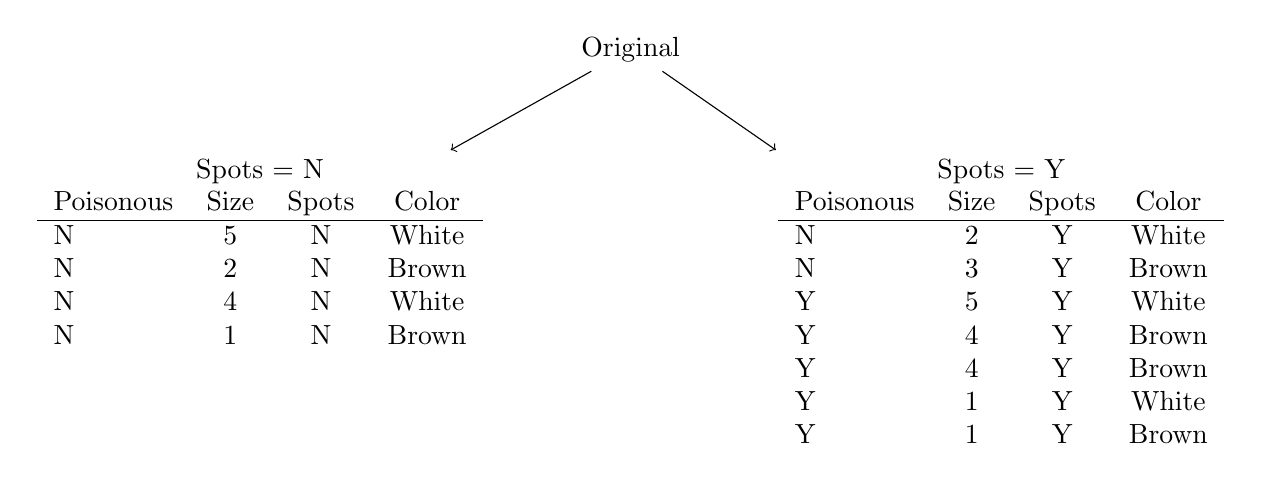
\begin{tikzpicture}
\node (developers){Original};
\node (probI)[below left=of developers,align=center]{Spots = N\\
	\begin{tabular}{l*{4}{c}r}
	Poisonous &Size &Spots &Color\\
	\hline
	N & 5 & N & White \\
	N & 2 & N & Brown \\
	N & 4 & N & White \\
	N & 1 & N & Brown \\
	\end{tabular}
};

\node (probIII)[below right=of developers,align=center]{Spots = Y\\
	\begin{tabular}{l*{4}{c}r}
	Poisonous &Size &Spots &Color\\
	\hline
	N & 2 &Y & White \\
	N & 3 &Y & Brown \\
	Y & 5 &Y & White \\
	Y & 4 &Y & Brown \\
	Y & 4 &Y & Brown \\
	Y & 1 &Y & White \\
	Y & 1 &Y & Brown \\
	
	\end{tabular}
};
% draw the connections
\draw[->] (developers)--(probI);
%\draw[->] (developers)--(probII);
\draw[->] (developers)--(probIII);
\end{tikzpicture}
\end{center}

\begin{sub}{6.1.2}
\end{sub}
Since the left node is already pure, we continue splitting on the right node.\\

a) Split on color:\\
i) color = white,  
$p_1 = \frac{2}{3} ,N_1 = 3,Q_1 = \frac{4}{9},  p_2 = \frac{3}{4},N_2 = 4, Q_2= \frac{6}{16}, N_1Q_1 + N_2Q_2  \approx 2.83$\\

b) Split on Size:\\
ii) Size $\leq$ 1, $p_1 = 0 ,N_1 = 2,Q_1 = 0,  p_2 = \frac{3}{5},N_2 = 5, Q_2= \frac{12}{25}, N_1Q_1 + N_2Q_2  \approx 2.4$\\
iii) Size $\leq$ 2, $p_1 = \frac{2}{3} ,N_1 = 3,Q_1 = \frac{4}{9},  p_2 = \frac{3}{4},N_2 = 4, Q_2= \frac{6}{16}, N_1Q_1 + N_2Q_2  \approx 2.83$\\
iv) Size $\leq$ 3, $p_1 = \frac{2}{4} ,N_1 = 4,Q_1 = \frac{1}{2},  p_2 = 1,N_2 = 3, Q_2= 0, N_1Q_1 + N_2Q_2  \approx 2$\\
v) Size $\leq$ 4 ,$p_1 = \frac{4}{6} ,N_1 = 6,Q_1 = \frac{4}{9},  p_2 = 1,N_2 = 1, Q_2= 0, N_1Q_1 + N_2Q_2  \approx 2.66$\\
The minimal weighted impurity measure is obtained by splitting on the Size $\leq$ 3.  \\

\begin{center}
	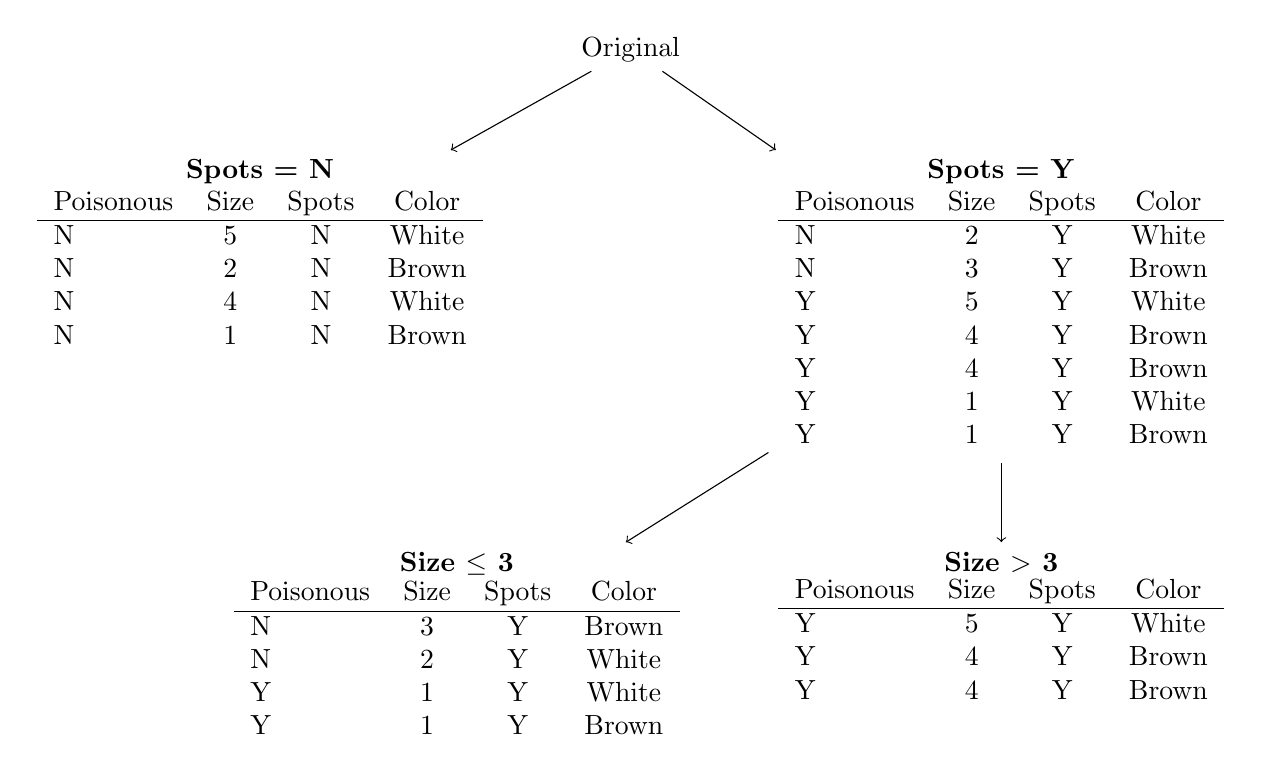
\begin{tikzpicture}
	\node (developers){Original};
	\node (probI)[below left=of developers,align=center]{\textbf{Spots = N}\\
		\begin{tabular}{l*{4}{c}r}
		Poisonous &Size &Spots &Color\\
		\hline
		N & 5 & N & White \\
		N & 2 & N & Brown \\
		N & 4 & N & White \\
		N & 1 & N & Brown \\
		\end{tabular}
	};
	
	\node (probIII)[below right=of developers,align=center]{\textbf{Spots = Y}\\
		\begin{tabular}{l*{4}{c}r}
		Poisonous &Size &Spots &Color\\
		\hline
		N & 2 &Y & White \\
		N & 3 &Y & Brown \\
		Y & 5 &Y & White \\
		Y & 4 &Y & Brown \\
		Y & 4 &Y & Brown \\
		Y & 1 &Y & White \\
		Y & 1 &Y & Brown \\
		
		\end{tabular}
	};
	
	\node (probIV)[below left=of probIII,align=center]{\textbf{Size $\leq$ 3} \\
		\begin{tabular}{l*{4}{c}r}
		Poisonous &Size &Spots &Color\\
		\hline
		N & 3 &Y & Brown \\
		N & 2 &Y & White \\
		Y & 1 &Y & White \\
		Y & 1 &Y & Brown \\
		\end{tabular}
	};
	
		
		\node (probV)[below =of probIII,align=center]{\textbf{Size $>$ 3} \\
			\begin{tabular}{l*{4}{c}r}
			Poisonous &Size &Spots &Color\\
			\hline
	
		Y & 5 &Y & White \\
		Y & 4 &Y & Brown \\
		Y & 4 &Y & Brown \\

			\end{tabular}
		};
		
	
	

	% draw the connections
	\draw[->] (developers)--(probI);
	%\draw[->] (developers)--(probII);
	\draw[->] (developers)--(probIII);
	\draw[->] (probIII)--(probIV);
	\draw[->] (probIII)--(probV);
	
	\end{tikzpicture}
\end{center}

Let region 1, 2, 3 be \{SPOT = N\}, \{SPOTS = Y, SIZE $\leq$ 3\}, \{SPOTS = N, SIZE $>$ 3\}\\
The predicted probability of poisonous is :\\
\begin{center}
	
	\begin{tabular}{l*{3}{c}r}
		Region & Prob of Poisonous & Prob of not Poisonous \\
		\hline
		
		1 & 0 \% & 100 \% \\
		2 & 50 \% & 50 \% \\
		1 & 100 \% & 0 \% \\		
	\end{tabular}
\end{center}


\begin{sub}{6.1.3}
\end{sub}

In the given dataset, the three features are binary, there will be at most 8 nodes. If we build the tree until all nodes are either pure or cannot be split further, the error will occurs on the data that have the same feature values but different Y values. In the given dataset, the training error happens in :
\begin{center}
	
	\begin{tabular}{l*{4}{c}r}
		Y & A & B &C \\
		\hline
		0 & 0 & 1 & 1 \\
		1 & 0 & 1 & 1 \\		
	\end{tabular}   \hspace{2in}	
		\begin{tabular}{l*{4}{c}r}
			Y & A & B &C \\
			\hline
			0 & 1 & 1 & 1 \\
			1 & 1 & 1 & 1 \\		
		\end{tabular}	
\end{center}

There will be 2 sample incorrectly labeled, therefore, the training error is $\frac{2}{11} \approx 18.1 \%$

\pagebreak
\begin{problem}{6.2 Investigating Impurity Measures}
\end{problem}


\begin{sub}{6.2.1}
\end{sub}

Misclassification rates:\\
Model A: $\frac{1}{4} \times \frac{1}{2} +\frac{1}{4} \times \frac{1}{2} = \frac{1}{4}$\\
Model B: $\frac{2}{6} \times \frac{6}{8} +0 \times \frac{2}{8} = \frac{1}{4}$\\

Cross-entropy: \\
Model A: $-\frac{3}{4}log(\frac{3}{4})\times \frac{1}{2} - \frac{1}{4}log(\frac{1}{4})\times \frac{1}{2} \approx 0.122 $\\
Model B: $-\frac{2}{6}log(\frac{2}{6})\times \frac{6}{8} - 1log(1)\times \frac{2}{6}\approx 0.119 $\\

Gini impurity:\\
Model A: $\frac{3}{4}\frac{1}{4}\frac{1}{2} + \frac{1}{4}\frac{3}{4}\frac{1}{2} =  \frac{3}{16} = 0.1875$\\
Model B: $\frac{1}{3}\frac{2}{3}\frac{6}{8} + 0 =  \frac{3}{16} \approx 0.1667$\\

Therefore, the Misclassification rates are identical for Model A and Model B, while the Cross-entropy and Gini impurity for Model B are less than that for Model A.

\section{7 Representer Theorem}
\begin{sub}{7.1}
\end{sub}
$m_0 = Proj_Mx$, and $||x||^2 = ||m_0||^2 + ||x - m_0||^2$\\
$||x|| = ||m_0|| \rightarrow ||x - m_0||^2 = 0$\\
$||x - m_0||^2 = <x - m_0,x - m_0>= 0$ iff $x-m_0 =\vec{0}$ by positive-definiteness of inner product. \\
Therefore $||x|| = ||m_0||$ only when $x=m_0 $

\begin{sub}{7.2}
\end{sub}
$R(\cdot)$ is strictly increasing, let M = $span(\psi(x_1),...,\psi(x_n) )$, assume $w^*$ is a minimizer, and w = Proj$_Mw^*$.\\ So $\exists \alpha \text{ s.t. } w = \sum\alpha_i\psi(x_i)  $\\

case 1: $||w|| = ||w^*||$\\
from 7.1, we know that if  $||w|| = ||w^*||$, then $x = m_0$\\
This immediately shows that w is a minimizer and w has the form $\sum\alpha_i\psi(x_i)  $\\

case 2: $||w|| < ||w^*||$\\
Since $R(\cdot)$ is strictly increasing, $R(||w||) < R(||w^*||)$\\
We know that $w^\perp  = w^* - w$ is orthogonal to M 
\begin{align}
<w^*,\psi(x_i)> = <w+ w^\perp,\psi(x_i)> = <w,\psi(x_i)>
\end{align}\begin{align}
L(<w^*,\psi(x_1)>,...,<w^*,\psi(x_n)>) = L(<w,\psi(x_1)>,...,<w,\psi(x_n)>)
\end{align}
Therefore, 
\begin{align}
J(w)   = R(||w||) + L(<w,\psi(x_1)>,...,<w,\psi(x_n)>) \\< R(||w^*||) + L(<w^*,\psi(x_1)>,...,<w^*,\psi(x_n)>) = J(w^*)
\end{align}
This contradict to the fact that $w^*$ is a minimizer. Therefore, this case is discarded.\\
In conclusion, only case 1 is possible, then we proved that all minimizers have the form $w = \sum\alpha_i\psi(x_i) $
\pagebreak


\begin{sub}{7.3}
\end{sub}
$w \in \Re^d$, let $A = \begin{pmatrix}
\psi_1(x_1)& \cdots &\psi_d(x_1)\\
\vdots &\vdots &\vdots\\
\psi_1(x_n)&\cdots & \psi_d(x_n)
\end{pmatrix}$ be the design matrix, b be the bias,$L(w) = Aw + b$\\
R and L are both convex, let $w_1, w_2 \in \Re^d$ and $0 \leq c \leq1$
\begin{align}
J(cw_1 + (1-c)w_2) = R(||cw_1 + (1-c)w_2||) + L(A(cw_1+(1-c)w_2)+b)
\end{align}
Since L is convex and $Aw+b$ is an affine function, $L(Aw+b)$ is convex.
\begin{align}
L(A(cw_1+(1-c)w_2)+b) \leq cL(Aw_1 +b)  + (1-c)L(Aw_2 +b)\end{align}
$||cw_1 + (1-c)w_2|| \leq c ||w_1|| + (1-c)||w_2||$, R is increasing and convex
\begin{align}
R(||cw_1 + (1-c)w_2||) \leq R(c ||w_1|| + (1-c)||w_2||) \leq cR(||w_1||) + (1- c)R(||w_2||)
\end{align}
eqn (17) and (18) together shows that 
\begin{align}
J(cw_1 + (1-c)w_2)  \leq cJ(w_1)+ (1-c)J(w_2)
\end{align}

This proves J is convex. 

\section{8 Ivanov and Tikhonov Regularization}

\begin{problem}{8.1 Tikhnov optimal implies Ivanov optimal}
\end{problem}
\begin{sub}{8.1.1}
\end{sub}
Since for some $\lambda > 0, f^*  = \underset{f \in \mathcal{F}}{\operatorname{argmin}}$ $ \phi(f) +\lambda \Omega(f)$, then :
\begin{align}
\nabla \phi(f^*) + \lambda \nabla\Omega(f^*) =0
\end{align}
Let $r = \Omega(f^*) > 0$, we need to show that :\\
$f^*$ is also a solution to $\underset{f \in \mathcal{F}}{\operatorname{argmin}}$ $\phi(f)$ s.t $\Omega(f) \leq \Omega(f^*)$\\
The Lagrangian to this Ivanov problem is  :
\begin{align}
L(f) = \phi(f) + \lambda(\Omega(f) - \Omega(f^*))
\end{align}
We claim that $f^*$ is a solution, by the first order condition :
\begin{align}
\nabla L(f^*) = \nabla \phi(f^*) + \lambda \nabla\Omega(f^*) &= 0\hspace{0.5in } \text{(from (20))}\\
\Omega(f^*) - \omega(f^*) &= 0
\end{align}
Therefore $f^*$ is also a Ivanov solution

\begin{problem}{8.2 Ivanov optimal implies Tikhonov optimal }
\end{problem}
\begin{sub}{8.2.1}
\end{sub}
The Lagrangian for Ivanov problem is :
\begin{align}
L(w,\lambda) = \phi(w) + \lambda(\Omega(w) - r)
\end{align}

\pagebreak

\begin{sub}{8.2.2}
\end{sub}
The duel problem is :
\begin{align}
g(\lambda) = \underset{w}{\operatorname{inf}} L(w,\lambda) = \underset{w}{\operatorname{min}} \hspace{0.05in} \phi(w) + \lambda(\Omega(w) - r)  
\end{align} 












\end{document}

